\documentclass[a4paper,11pt]{article}

%%%%%%%%%%%%%%%%%%%%%%%%%%%%%%%%%%%%%%%%%%%%%%%%%%%%%%%%%%%%%%%%%%%%%%%%
% Paquetes utilizados
%%%%%%%%%%%%%%%%%%%%%%%%%%%%%%%%%%%%%%%%%%%%%%%%%%%%%%%%%%%%%%%%%%%%%%%%

% Gráficos complejos
\usepackage{graphicx}
\usepackage{caption}
\usepackage{subcaption}
\usepackage{placeins}

% Soporte para el lenguaje español
\usepackage{textcomp}
\usepackage[utf8]{inputenc}
\usepackage[T1]{fontenc}
\DeclareUnicodeCharacter{B0}{\textdegree}
\usepackage[spanish]{babel}

% Código fuente embebido
\usepackage{listings}

% PDFs embebidos para el apéndice
\usepackage{pdfpages}

% Matemáticos
\usepackage{amssymb,amsmath}

% Tablas complejas
\usepackage{multirow}

% Formato de párrafo
\setlength{\parskip}{1ex plus 0.5ex minus 0.2ex}

%%%%%%%%%%%%%%%%%%%%%%%%%%%%%%%%%%%%%%%%%%%%%%%%%%%%%%%%%%%%%%%%%%%%%%%%
% Título
%%%%%%%%%%%%%%%%%%%%%%%%%%%%%%%%%%%%%%%%%%%%%%%%%%%%%%%%%%%%%%%%%%%%%%%%

% Título principal del documento.
\title{\textbf{Trabajo Práctico 2: Profiling y optimización}}

% Información sobre los autores.
\author{
  Andrés Gastón Arana, \textit{P. 86.203}                          \\
  \texttt{and2arana@gmail.com}                                     \\
  Sergio Matías Piano, \textit{P. 85.191}                          \\
  \texttt{smpiano@gmail.com}                                       \\ [2.5ex]
  \normalsize{2do. Cuatrimestre de 2012}                           \\
  \normalsize{66.20 Organización de Computadoras}                  \\
  \normalsize{Facultad de Ingeniería, Universidad de Buenos Aires}
}
\date{}

%%%%%%%%%%%%%%%%%%%%%%%%%%%%%%%%%%%%%%%%%%%%%%%%%%%%%%%%%%%%%%%%%%%%%%%%
% Documento
%%%%%%%%%%%%%%%%%%%%%%%%%%%%%%%%%%%%%%%%%%%%%%%%%%%%%%%%%%%%%%%%%%%%%%%%

\begin{document}

% ----------------------------------------------------------------------
% Top matter
% ----------------------------------------------------------------------
\thispagestyle{empty}
\maketitle

\begin{abstract}

  Este informe sumariza el desarrollo del trabajo práctico 2 de la materia
  Organización de Computadoras (66.20) dictada en el segundo cuatrimestre de
  2012 en la Facultad de Ingeniería de la Universidad de Buenos Aires. El mismo
  consiste en la optimización de un sistema de simulación con énfasis en el
  análisis de perfilado y aprovechamiento de cache.

\end{abstract}

\clearpage

% ----------------------------------------------------------------------
% Tabla de contenidos
% ----------------------------------------------------------------------
\tableofcontents
\clearpage


% ----------------------------------------------------------------------
% Desarrollo
% ----------------------------------------------------------------------
\part{Desarrollo}

\section{Introducción}

\section{Profiling inicial}

\section{Optimizaciones propuestas}

\section{Profiling optimizaciones}

\section{Conclusiones}


\clearpage

\part{Apéndice}
\appendix

\section{Enunciado original}\label{sec:enunciado}
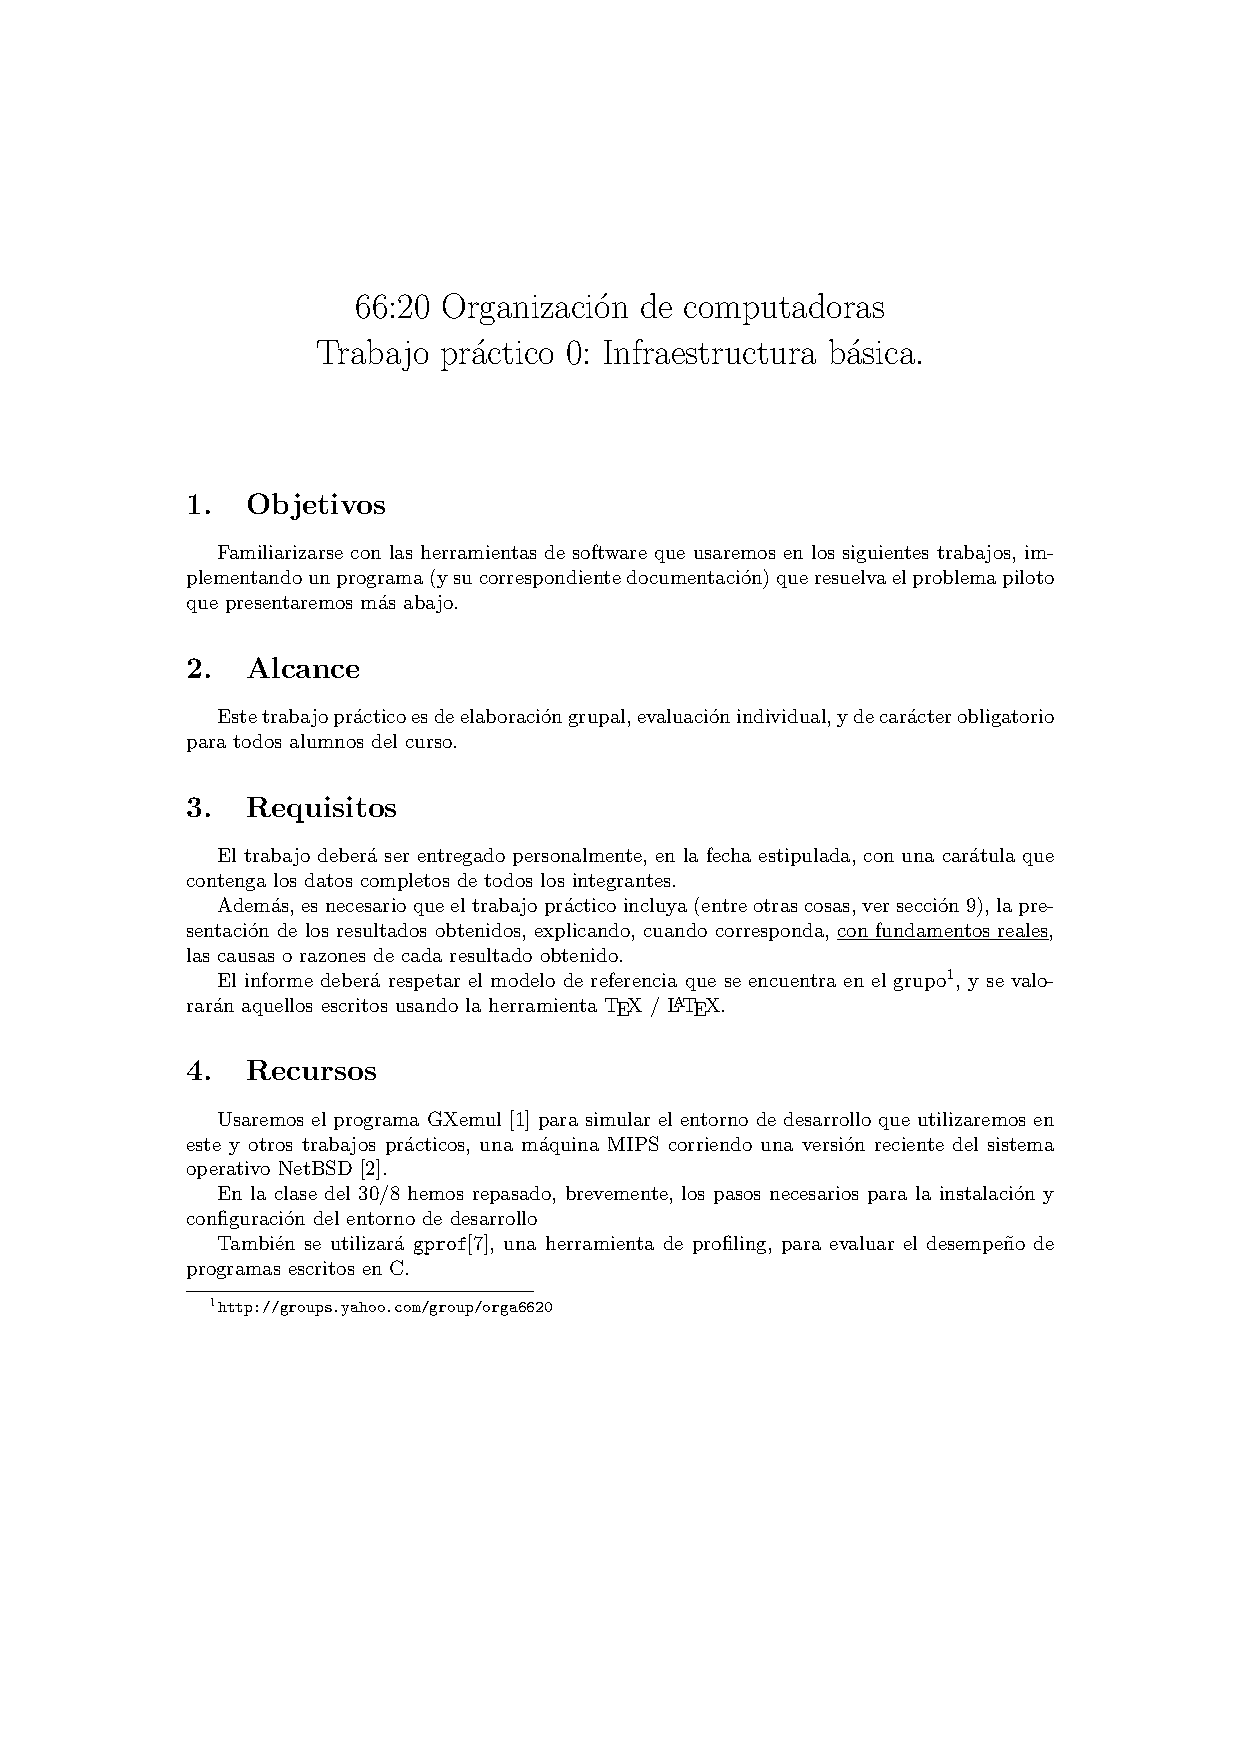
\includepdf[pages={-}]{docs/enunciado.pdf}

\clearpage
\section{README del material digital}\label{sec:readme}
\includepdf[pages={-}]{build/doc/README.pdf}

\clearpage
\section{Código fuente optimizaciones}\label{sec:source}
\clearpage
\definecolor{gray}{rgb}{0.5,0.5,0.5}
\lstset{
  title=\lstname,
  basicstyle=\footnotesize,
  showspaces=false,
  showstringspaces=false,
  breaklines=true,
  commentstyle=\color{gray},
  numbers=left,
  numberstyle=\tiny\color{gray},
  numbersep=5pt,
  frame=single
}

\lstinputlisting{source/wator.c}

\end{document}

